% !TEX root = ../thesis.tex

\chapter{Circuit Enumeration}\label{apx:chp_enumeration}

%=================================================
\section{Subtleties in the Enumeration}\label{app:subtleties}
%=================================================
Enumerating all possible circuits is a formidable task. Although we have carried out this enumeration, it relies on several assumptions. In this appendix, we discuss subtleties that fall outside the scope of the main study and may affect the circuits we enumerate. These include stray capacitances and inductances, readout resonators, transmission lines, and Purcell filters. The list is not exhaustive, and no single study could address all such complications.

% ------------------------------------------------
\subsection{Ground Placement and Circuit Equivalence}\label{sec:gnd}
% ------------------------------------------------
Our enumeration procedure does not assign any nodes to ground, although the choice of ground can significantly change a circuit's Hamiltonian. When modeling circuits in \cref{sec:optimization}, we choose to include capacitive coupling between each node and ground.

Ground placement can also change the effective circuit topology. Consider the two circuits in \cref{fig:ground_transformation}(a) and (b), which have three and four nodes, respectively. If we ground one node in \cref{fig:ground_transformation}(a) and two nodes in \cref{fig:ground_transformation}(b), both reduce to a circuit that resembles galvanically coupled transmons. As a result, including grounds can cause our procedure to over-count unique circuits. For a graph with $N$ nodes, there are
$\sum_{k=1}^{N-1}\binom{N}{k} = 2^N - 2$
ways to ground one or more nodes. One could enumerate these possibilities and identify equivalent configurations by adding a ground ``color'' to the graph-isomorphism procedure described in \cref{sec:CirEnumAlg}. However, grounding multiple nodes effectively reduces the number of nodes in the circuit. These reduced circuits are therefore not new configurations and already appear in the enumeration of smaller circuits.

\begin{figure}[htbp]
\centering 
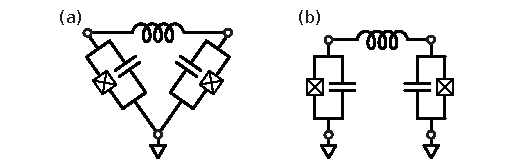
\includegraphics[width=\colfigwidth]{chapter-3-enumeration/figs/grounding.pdf}
\caption{Illustration of how the number and placement of ground nodes can induce circuit isomorphism. Circuit (a) has three nodes, while circuit (b) has four. The two circuits become equivalent when the indicated one node in (a) and two nodes in (b) are grounded.}\label{fig:ground_transformation}
\end{figure}


%-------------------------------------------
\subsection{Ambiguities Related to SQUIDs and Linearization}\label{sec:SQUIDs}
%-------------------------------------------
We did not include superconducting quantum interference devices (SQUIDs) or tunable inductors built from flux-biased SQUIDs in our enumeration. In a sense, any Josephson junction in our enumeration could be viewed as a split junction, i.e., a SQUID. Likewise, any linear inductor could be viewed as a linearized SQUID; see \cref{fig:SQUID_amb}. These distinctions matter at the Hamiltonian level because SQUID-based elements introduce additional tunable terms, such as $(\phi-\phi_{\rm ext})^2$ and $\cos(\phi-\phi_{\rm ext})$.

Flux bias can also be used to engineer effective cubic or quartic terms \cite{Frattini_snail_2017, Quarton2021}. A standard example is the SNAIL \cite{Frattini_snail_2017}. The SNAIL consists of several Josephson junctions in a series-parallel arrangement. By tuning the external flux, one can isolate selected powers of the phase operator, $\phi^n$. To include such effects, one could introduce new effective dipole elements into the enumeration. This is a direction that could reveal new circuit classes, but it lies beyond the scope of our present procedure.

\begin{figure}[htbp]
\centering 
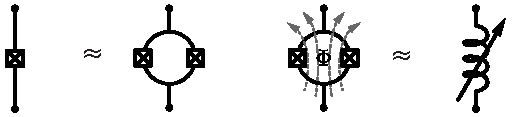
\includegraphics[width=\colfigwidth]{chapter-3-enumeration/figs/squid.pdf}
\caption{Flux-tunable elements not included explicitly in our enumeration.}\label{fig:SQUID_amb}
\end{figure}



%-------------------------------------------
\subsection{Charge and Flux Bias} \label{sec:charge_flux_bias}
% ----------------------------------------
We do not include charge and flux biases in the enumeration itself, although they do appear in the optimization over unique circuits; see \cref{fig:flux_n_charge_bias}. These biases can distinguish circuits that otherwise belong to the same Hamiltonian class, as defined in \cref{sec:HamEnum}.

\begin{figure}[htbp]
\centering 
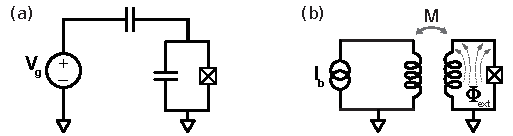
\includegraphics[width=\colfigwidth]{chapter-3-enumeration/figs/voltage_flux.pdf}
\caption{Examples of (a) a charge-bias circuit and (b) a flux-bias circuit, neither of which is included explicitly in the enumeration.}\label{fig:flux_n_charge_bias}
\end{figure}

To see this, consider the circuit Hamiltonian
\begin{align}
    H = \frac{1}{2}(Q - Q_g)^T C^{-1}(Q - Q_g) + U(\Phi, \Phi_{\rm ext}),
\end{align}
where $Q$ is the vector of node charges, $\Phi$ is the vector of node fluxes, $C^{-1}$ is the inverse capacitance matrix, and $Q_g$ is a vector of gate charges. We can identify a separate circuit and coupling Hamiltonian:
\begin{align}
    H_{\rm circuit} &= \frac{1}{2}Q^T C^{-1}Q + U(\Phi) \\
    H_{\rm coupling} &= Q^T C^{-1} C_V V + U(\Phi, \Phi_{\rm ext}).
\end{align}
In \cref{sec:HamEnum}, we classify circuits using only $H_{\rm circuit}$. This is equivalent to setting $Q_g = 0$ and  $\Phi_{\rm ext} = 0$ in the full Hamiltonian. Circuits in the same Hamiltonian class may still differ in $H_{\rm coupling}$. Those differences determine how the system can be controlled and may also affect decoherence. %A full analysis of charge and flux bias should therefore be left to future work.
A classification that also incorporates these bias-dependent coupling Hamiltonians is left to future work.

% ----------------------------------------
\subsection{Circuit Elements Not Considered} \label{subsec:elems considered}
% ----------------------------------------
We did not include several elements that appear in the superconducting-circuit literature, such as resistors and three-terminal devices like circulators. Two cases deserve further comment: quantum phase-slip junctions and multiport nonreciprocal devices; see \cref{fig:QPS_mulitport}.


\begin{figure}[htbp]
\centering 
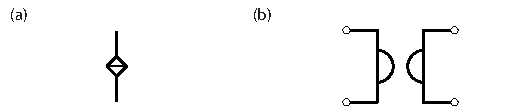
\includegraphics[width=\colfigwidth]{chapter-3-enumeration/figs/qps_gyrator.pdf}
\caption{QPS elements and multiport/multiterminal devices.}\label{fig:QPS_mulitport}
\end{figure}

A quantum phase-slip junction (QPS)~\cite{Mooij_QPS_2006} is effectively a nonlinear capacitor and is the electrical dual of the Josephson junction. Although QPS has not yet been realized unequivocally in experiment, we excluded it from the main study for a more practical reason: modern superconducting-circuit analysis packages do not support it. That would sharply limit the analysis of the resulting circuits. Even so, adding a new two-terminal device is straightforward at the level of \textit{circuit} enumeration. To begin exploring circuits with QPS, we carried out a secondary enumeration of circuits with up to four nodes using all fifteen combinations of capacitor (\verb|C|), inductor (\verb|L|), Josephson junction (\verb|J|), and QPS (\verb|Q|).
\begin{align*}
\texttt{C},\, \texttt{J},\, \texttt{L},\, \texttt{Q},\, &\texttt{JC},\, \texttt{CL},\, \texttt{QC},\, \texttt{JL},\,\texttt{JQ},\, \texttt{QL},\, \\ 
\texttt{JCL},\, \texttt{JQC}&, \, \texttt{QCL}, \, \texttt{JQL}, \textrm{and}\, \texttt{JQCL}.
\end{align*}
\Cref{tab:qps_enum} gives the resulting number of unique circuits.

\begin{table}[htbp]
\setlength{\tabcolsep}{15pt}
\begin{tabular}{@{}ccc@{}}
\toprule
Nodes \,\,      &  Circuits&  Unique Nonlinear Circuits  \\ \toprule
2                  & 15          &   12          \\ \midrule
3                  & 3600        &   736         \\ \midrule
4                  & 12,258,000    &   712,682 \\ \bottomrule
\end{tabular}
 \caption{Number of enumerated circuits as a function of node count for circuits built from \texttt{C}, \texttt{L}, \texttt{J}, and \texttt{Q}. Column 1 gives the number of nodes. Column 2 gives the naive count, $15^{N_E}$, summed over all base graphs for that node count (see \cref{fig:basegraph_grid}). Column 3 gives the number of unique nonlinear circuits containing at least one Josephson junction or one QPS element.}\label{tab:qps_enum}
\end{table}

Nonreciprocal devices such as circulators and gyrators raise two separate issues: nonreciprocity and multiport structure. The first is that consistent quantization of nonreciprocal devices has only recently been developed~\cite{parra-rodriguez2023}, and current software packages do not yet support it. The second is that multiport devices would add substantial overhead to the enumeration itself. Their circuit topologies would need to be represented by directed hypergraphs rather than undirected graphs. That would increase the number of possible configurations and prevent us from using widely available precomputed lists of nonisomorphic simple graphs, since comparable lists for hypergraphs are not generally available.


\subsection{Eliminating Single-Node Capacitive and Inductive Islands}\label{app:details:islands}

We do not consider circuits that contain a single node connected only to capacitors or only to inductors. In such cases, one can construct an equivalent circuit with one fewer node and the same equations of motion. We show below how to identify the required effective capacitance or inductance from the circuit Lagrangian. This construction is equivalent to a generalized delta-Y, or star-mesh, transformation \cite{rosen_new_1924}.


Consider a subcircuit of $n$ capacitors, $[C_1, C_2, \dots, C_n]$, that meet at a central node. Additional capacitive connections may already exist between the outer terminals.

The central-node variable is a free variable, but it is coupled to the outer nodes, which may themselves be dynamical. We now follow the procedure in \cref{app:var_trans:decouple} to decouple this free variable and derive reduced dynamics that do not depend on the central node.

We first split the node flux variables into two parts,
\begin{align*}
\phi = \begin{pmatrix}
    \phi_1 \\
    \phi_2
\end{pmatrix}.
\end{align*}
where $\phi_1$ contains the outer nodes and $\phi_2$ contains the inner node variable. We likewise partition the capacitance matrix into blocks for the outer nodes $C_{11}$, inner nodes $C_{22}$, and their couplings $C_{21}, C_{12}$:
\begin{align*}
    C &= \begin{pmatrix}
    C_{11} & C_{12} \\
    C_{21} & C_{22}
\end{pmatrix}.
\end{align*}
Given the structure of the circuit,
\begin{align}
\begin{split}
    C_{11} &= \rm diag([C_1, C_2, \dots, C_n]) + C_0 \\
    C_{22} &= \sum_{i=1}^n C_i = C_\Sigma \\
    C_{21} &= C_{12}^T = \rm row([C_1, C_2, \dots, C_n]),
\end{split}
\end{align}
where $\rm diag$ denotes a diagonal matrix and $\rm row$ a row vector. Here $C_i$ is the capacitance between outer node $i$ and the central node, while $C_0$ contains the capacitances that connect the outer ports to one another or to the rest of the circuit.

The modified capacitance matrix
\begin{align}
    \tilde{C} = C_{11} - C_{12}C_{22}^{-1}C_{21} = C/C_{22}
\end{align}
defines a reduced system dynamics. To calculate $\tilde{C}$, first consider the entries
\begin{align*}
    [C/C_{22}]_{ij} = [\begin{pmatrix}
        C_1 \\
        \vdots \\
        C_n
    \end{pmatrix} \frac{1}{C_\Sigma}\begin{pmatrix}
        C_1 & \dots & C_n
    \end{pmatrix}]_{ij} = \frac{C_iC_j}{C_\Sigma}.
\end{align*}
The diagonal entries are therefore
\begin{align}\label{eq:reduced_diagonal}
    [\tilde{C}]_{ii} = [C_0]_{ii} + C_i - \frac{C_i^2}{C_\Sigma} = [C_0]_{ii} + \frac{\sum_{i\neq j} C_iC_j}{C_\Sigma}
\end{align}
and off-diagonal entries are
\begin{align}
    [\tilde{C}]_{ij} = [C_0]_{ij} - \frac{C_iC_j}{C_\Sigma}.
\end{align}

It follows that the same Lagrangian can be realized by a circuit with no inner node and an added capacitance $\frac{C_iC_j}{C_\Sigma}$ between outer nodes $i$ and $j$. In the special case of one inner node and one outer node, that is, a dangling capacitor or inductor attached to a single node, \cref{eq:reduced_diagonal} reduces to
$[\tilde{C}]_{ii} = [C_0]_{ii} + C_i - C_i^2/C_\Sigma = [C_0]_{ii}$. The dangling element therefore does not affect the dynamics, as no current can flow through that branch.

We omit the corresponding derivation for a node connected only to inductors, as it is identical to the capacitive case.


\section{Variable Transformation Details}\label{app:var_trans}
\subsection{Choice of ``\Canonical'' Coordinates}
The goal of this section is to define a set of ``\canonical'' coordinates for a general superconducting circuit made of capacitors, inductors, and Josephson junctions. Our method generates a transformation to bring any circuit Lagrangian into a standard form, which we use to categorize circuits into ``Hamiltonian classes.'' 
Hamiltonian classes consist of Hamiltonians with the same functional form but different parameter values. 

The definition of our \canonical\ coordinates is motivated by a desire for minimally coupled circuit modes, without a dependence on underlying circuit parameters. The underlying transformation algorithm is flexible and could be used to generate different choices of ``\canonical'' coordinates.

For a general circuit, we impose the following requirements.
\begin{enumerate}
\item[(1)] Maximize the number of non-extended modes, identifying compact, harmonic, and non-dynamical modes wherever possible.
\item[(2)] Non-dynamical modes must not couple to dynamical modes.
\item[(3)] All dynamical coordinates must be parameter-independent linear combinations of node variables.
\item[(4)] Compact coordinates form an $n$-dimensional cubic unit cell, with charges quantized in units of Cooper pairs. Thus, the lattice vectors of the periodic potential are the standard basis vectors \cite{rajabzadehAnalysisArbitrarySuperconducting2023}.
\end{enumerate}
Within the constraints of the above requirements, some freedom in the choice of coordinates remains. We fix a unique choice by imposing the following criteria, in order of priority:

\begin{enumerate}
\item[(a)] Minimize nonlinear inter-mode coupling, measured by the off-diagonal support of 
$J = \sum_i E_{J,i}\,\omega_{J,i}\omega_{J,i}^T$, where $\omega_{J,i}$ denotes the $i$th junction incidence vector.
\item[(b)] Minimize linear inter-mode coupling, defined by the number of nonzero off-diagonal entries in the transformed inverse capacitance ($C^{-1}$) and susceptance ($L^*$) matrices. In case of a tie, prioritize minimizing inductive coupling. As a further tiebreaker, prefer transformations with fewer off-diagonal terms when all circuit parameters are taken to be identical.
\item[(c)] Ensure integer arguments in cosine potentials of extended modes (e.g., $\cos(2\varphi)$, not $\cos(1.45\varphi)$). Coefficients are chosen to minimize the $\ell_1$ norm of the transformed junction incidence matrix.
\end{enumerate}

Finally, we impose a preferred ordering of variable labels. Specifically, we order the coordinate vector as
$\Phi = (\Phi^{c}, \Phi^{e}, \Phi^{h}, \Phi^{\rm fr,fz,cy})^T$,
with a vector of compact variables first, followed by extended, harmonic, and non-dynamical variables.

\subsection{Generating a ``\Canonical'' Transformation}

The requirements of our ``\canonical'' coordinates motivate a sequence of three linear transformations. The first transformation splits modes into different types and addresses requirements (1) and (4). The second transformation enforces requirement (2) by removing any residual coupling between dynamical and non-dynamical variables. 
Both steps can be carried out without violating the parameter-independence requirement of (3).
Finally, the third transformation performs the minimization described in (a) and (b), again subject to the parameter dependence requirement of (3). 
An implementation of this transformation is included in our code \cite{sircuitenum_repo}.



\subsubsection{Separate Mode Types}

For a circuit with capacitance matrix $C$, susceptance matrix $L^*$, and junction incidence matrix $\omega_J$, the Lagrangian is written in terms of node flux variables $\Phi$ as
\begin{align}\label{eq:node_lagrangian}
    \mathcal{L}(\Phi, \dot \Phi) = \frac{1}{2}\dot\Phi^TC\dot\Phi &- \frac{1}{2}\Phi^TL^*\Phi  \nonumber \\ &+ \sum_iE_{J,i}\cos\left(\frac{2\pi}{\Phi_0}\omega_{J,i}^T\Phi\right),
\end{align}
neglecting charge offset and external flux. Here $\Phi_0$ is the superconducting magnetic flux quantum. $E_{J,i}$ and $\omega_{J,i}$ are the Josephson energy and incidence matrix column corresponding to junction $i$. Each $\omega_J$ column represents a Josephson junction, with a $\pm1$ at entries corresponding to connected nodes. For example, a three-node circuit with a junction connecting nodes two and three would have $\omega_J = \{0,1,-1\}$ or $\omega_J = \{0,-1,1\}$. Because cosine is an even function, the choice of head/tail does not matter, though consistency is key when considering time-dependent flux drives \cite{rajabzadehAnalysisArbitrarySuperconducting2023}. Note that the linear terms can also be expressed with incidence matrices, such as $\dot\Phi^TC\dot\Phi = \sum_i(C_i\omega_{C,i}^T\dot \Phi)^2$.


We define a new set of coordinates $\tilde{\Phi}$ by a linear transformation of the node flux variables,
$\tilde{\Phi} = Z^{-1}\Phi$.
Although the inverse may appear unconventional, this choice ensures that the capacitance matrix $C$, the susceptance matrix $L^*$, and the junction incidence vectors $\omega_J$ transform with $Z$. This is seen by substituting $\Phi = Z\tilde{\Phi}$ into \cref{eq:node_lagrangian}, which yields
\begin{align}\label{eq:tilde_lagrangian}
    %\mathcal{L}(\Phi, \dot \Phi) &= \dot\Phi^T(Z^{-1})^TZ^TCZZ^{-1}\dot \Phi - \Phi^T (Z^{-1})^TZ^T L^*ZZ^{-1}\Phi  \nonumber \\ & \quad + \sum_iE_{J,i}\cos(\frac{2\pi}{\Phi_0}\omega_{J,i}^TZZ^{-1}\Phi) \nonumber \\
    \mathcal{L}(\tilde \Phi, \dot{\tilde\Phi}) &= \frac{1}{2}\dot{\tilde\Phi}^TZ^TCZ\dot{\tilde\Phi} - \frac{1}{2}\tilde \Phi^TZ^T L^*Z\tilde \Phi  \nonumber \\ & \quad + \sum_iE_{J,i}\cos\left(\frac{2\pi}{\Phi_0}\omega_{J,i}^T Z \tilde \Phi\right)
\end{align}
and can now be written in terms of transformed matrices
\begin{align}
    &\tilde C = Z^TCZ, \quad \tilde{L}^* = Z^TL^*Z, ~~\textrm{and}~~ \tilde \omega_J^T = \omega_J^T Z ~.
\end{align}


For circuits with capacitors, inductors, and Josephson junctions with intrinsic capacitance, six distinct modes arise\footnote{Consistently treating Josephson junctions without intrinsic capacitance can lead to multi-valued constraints and remains an area of active research~\cite{rymarz_consistent_2023, Eguisquiz_Reply_Consistent_2025, Eguisquiz_Comment_Consistent_2025}.}. Three are dynamical: compact (cosine potential), extended (cosine + quadratic potential), and harmonic (quadratic potential). Three are non-dynamical: free (kinetic only), frozen (potential only), and cyclic (absent from the Lagrangian).

We define coordinates $\Phi_1$ = $\{\Phi_1^{\rm c}, \Phi_1^{\rm e}, \Phi_1^{\rm h},        \Phi_1^{\rm fr}, \Phi_1^{\rm fz} , \Phi_1^{\rm cy}\}^T$ that contain blocks corresponding to different mode types.\footnote{A circuit has as many modes as active circuit nodes, so for any given circuit, many of these blocks will be of dimension zero.} The corresponding transformation can be written as $\Phi = Z_1\Phi_1$, or
\begin{align}
     &\begin{pmatrix}
        \phi_0 \\ \phi_1 \\ \vdots \\ \phi_{n-1} \\ \phi_n
    \end{pmatrix}
    = Z_1 
    \begin{pmatrix}
       \Phi_1^{\rm c} \\\Phi_1^{\rm e} \\ \Phi_1^{\rm h} \\
       \Phi_1^{\rm fr} \\\Phi_1^{\rm fz} \\ \Phi_1^{\rm cy}
    \end{pmatrix}.
\end{align}
Here $\phi_i$ denotes a circuit node flux variable. The columns of the transformation $Z_1$ impose restrictions on the nature of the corresponding variables. To see this, consider $Z_1$ as blocks corresponding to different variable types
\begin{align}
Z_1 
    \begin{pmatrix}
       \Phi_1^{\rm c} \\\Phi_1^{\rm e} \\ \Phi_1^{\rm h} \\
       \Phi_1^{\rm fr} \\\Phi_1^{\rm fz} \\ \Phi_1^{\rm cy}
    \end{pmatrix}&= \begin{pmatrix}
        Z_1^{\rm c} & Z_1^{\rm e} & Z_1^{\rm h} & Z_1^{\rm fr} & Z_1^{\rm fz} & Z_1^{\rm cy}
    \end{pmatrix}
    \begin{pmatrix}
       \Phi_1^{\rm c} \\\Phi_1^{\rm e} \\ \Phi_1^{\rm h} \\
       \Phi_1^{\rm fr} \\\Phi_1^{\rm fz} \\ \Phi_1^{\rm cy}
    \end{pmatrix} \nonumber \\
    &= (
       Z_1^{\rm c}\Phi_1^{\rm c} +Z_1^{\rm e}\Phi_1^{\rm e} + Z_1^{\rm h}\Phi_1^{\rm h} + \nonumber \\
    & \quad ~~~   Z_1^{\rm fr}\Phi_1^{\rm fr} + Z_1^{\rm fz}\Phi_1^{\rm fz} + Z_1^{\rm cy}\Phi_1^{\rm cy}
    ).
\end{align}
For example, consider the requirements to define a harmonic coordinate. It must not have a cosine potential, which requires $\Phi_1^{\rm h}$ never appear in any $\cos$ term of \cref{eq:node_lagrangian}. Equivalently, $\omega_{J}^TZ\Phi_1 = \omega_{J}^T(
       Z_1^{\rm c}\Phi_1^{\rm c} +Z_1^{\rm e}\Phi_1^{\rm e} + Z_1^{\rm h}\Phi_1^{\rm h} + Z_1^{\rm fr}\Phi_1^{\rm fr} + Z_1^{\rm fz}\Phi_1^{\rm fz} + Z_1^{\rm cy}\Phi_1^{\rm cy}
    )$
must not depend on $\Phi_1^{\rm h}$. This condition is satisfied if and only if
\begin{align}\label{eq:omegaj_null}
    \omega_J^TZ_1^{\rm h} = 0 \quad \textrm{or} \quad \textrm{col}(Z_1^{\rm h}) \in \textrm{null}(\omega_J^T),
\end{align}
where the notation $\textrm{col}(A)$ denotes the set of all linear combinations of the columns of $A$, and $\textrm{null}(A)$ means the set of vectors $x$ for which $Ax=0$.
So \cref{eq:omegaj_null} means all columns of $Z_1^{\rm h}$ are inside the nullspace of $\omega_J^T$. A harmonic mode must also have a quadratic potential and momentum, which requires
\begin{align}
    \textrm{col}(Z_1^{\rm h}) \notin \textrm{null}(\omega_L^T) \quad \textrm{and} \quad \textrm{col}(Z_1^{\rm h}) \notin \textrm{null}(\omega_C^T)~,
\end{align}
for inductor and capacitor incidence matrices $\omega_L$ and $\omega_C$.

\begin{figure}[htbp]
\centering
\resizebox{0.85\columnwidth}{!}{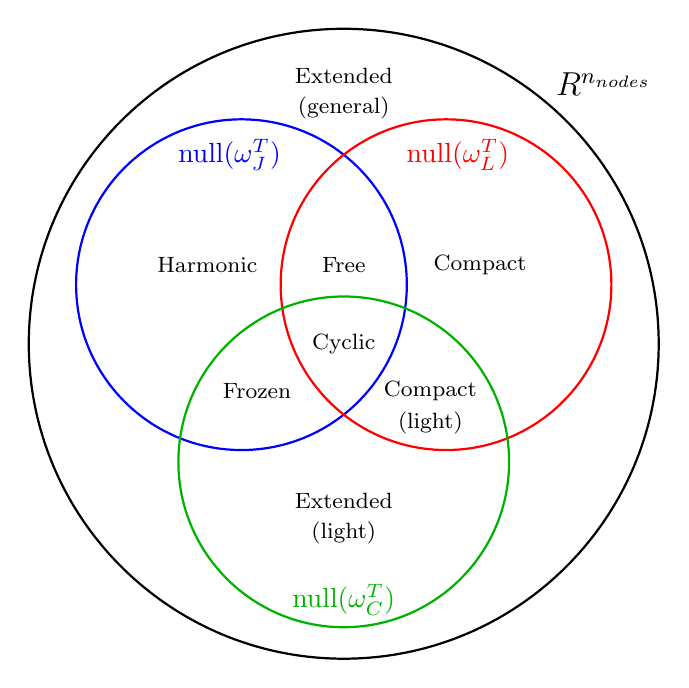
\begin{tikzpicture}

% Main enclosing circle
\draw[thick] (0,0) circle (4.0);
\node at (3.3, 3.3) {\large \(\mathbb{R}^{n_{\text{nodes}}}\)};
\node at (0,3.4) {\footnotesize Extended};
\node at (0, 3.4-0.4) {\footnotesize(general)};
%\node at (3.2*0.866+0.1,3.2*-0.5+0.25) {\footnotesize Extended};
%\node at (3.2*0.866+0.1, 3.2*-0.5-0.4+0.25) {\footnotesize(general)};

% Blue circle (N(W_J)) 30 degrees cosx = 0.866
\draw[thick, blue] (1.5*-0.866,1.5*0.5) circle (2.1);
\node[blue] at (-1.45, 2.4) {\normalsize \({\mathrm{null}(\omega_J^T)}\)};
\node at (2*-0.866,2*0.5) {\footnotesize Harmonic};

% Red circle (N(W_L)) 30 degrees cosx = 0.866, sin30 = 0.5
\draw[thick, red] (1.5*0.866,1.5*0.5) circle (2.1);
\node[red] at (1.45, 2.4) {\normalsize \({\mathrm{null}(\omega_L^T)}\)};
\node at (2*0.866,2*0.5) {\footnotesize Compact};

% Green circle (N(W_C)) cos270 = 0
\draw[thick, green!70!black] (1.5*0,1.5*-1) circle (2.1);
\node[green!70!black] at (0,-3.25) {\normalsize \(\mathrm{null}(\omega_C^T)\)};
\node at (0, -2) {\footnotesize Extended};
\node at (0, -2.4) {\footnotesize (light)};

% Intersections
\node at (0.0, 1.0) {\footnotesize Free};
\node at (0, 0.0) {\footnotesize Cyclic};
\node at (-1.1, -0.60) {\footnotesize Frozen};
\node at (1.1, -0.60) {\footnotesize Compact};
\node at (1.1, -1.00) {\footnotesize (light)};

\end{tikzpicture}
}
\caption{Types of modes in superconducting circuits made of pure capacitors, pure inductors, and Josephson junctions with intrinsic capacitance. The columns of $Z_1^{m}$ for a given mode type $m$ are placed within the null spaces of the incidence matrices $\omega_J^T$, $\omega_L^T$, and $\omega_C^T$. Light indicates a small capacitance or ``mass'' from only the intrinsic junction capacitance.}\label{fig:mode_diagram}
\end{figure}

Our algorithm incorporates the analogous requirements on $\textrm{null}(\omega_J)$, $\textrm{null}(\omega_L)$, and $\textrm{null}(\omega_C)$ shown in \cref{fig:mode_diagram}, which enable the automatic construction of $Z_1$. We describe the procedure below.
\begin{enumerate}
    \item[(1)] Construct incidence matrices $\omega_J, \omega_C, $ and $\omega_L$.
    \item[(2)] Determine the dimension of each zone in \cref{fig:mode_diagram} to identify the modes present.
    \item[(3)] For non-compact modes $m$, select any valid choice of $Z_1^m$. These columns will be redefined later to minimize inter-mode coupling.
    \item[(4)] For compact modes $c$, the desired lattice vectors are achieved when a subset of rows in $\omega_J^TZ_1^c$ is equal to the identity matrix. Beginning with any choice of $Z_1^c$ that respects \cref{fig:mode_diagram}, all $Z_1^c$ with desired lattice vectors can be obtained by inverting different linearly-independent sets of rows of $\omega_J^TZ_1^c$.
\end{enumerate}

\subsubsection{Decouple Non-Dynamical Modes} \label{app:var_trans:decouple}
After the first transformation, dynamical modes may be linearly coupled to non-dynamical modes. It is always possible to define a transformation that decouples them \cite{ding_free-mode_2021}. We can define this secondary transformation $\Phi_1 = Z_2\Phi_2$ in terms of the dynamical (c, e, h) and non-dynamical (fr,fz,cy) blocks of $\Phi_1$
\begin{align}
    \begin{pmatrix}
        \Phi_1^{\rm c,e,h} \\ \Phi_1^{\rm fr,fz,cy}
    \end{pmatrix} = Z_2 \begin{pmatrix}
        \Phi_2^{\rm c,e,h} \\ \Phi_2^{\rm fr,fz,cy}
    \end{pmatrix}.
\end{align}
The only choice of $Z_2$ that does not alter the definitions of dynamical variables is 
\begin{align}
    Z_2 = \begin{pmatrix}
    I & 0 \\
    M & I
\end{pmatrix} ~,
\end{align}
with $M= -C_{22}^{-1}C_{21}$ or $M = -(L^*_{22})^{-1}L^{*}_{21}$ depending on whether the dynamical modes are coupled by charge or flux. Block 1 denotes dynamical modes (c, e, h), and block 2 denotes non-dynamical modes (fr, fz, cy). If coupling occurs through both, the two transformations are applied in series. It can be shown that the decoupling transformation $Z_2$ is unique up to redefining the non-dynamical modes. 

It is worth noting that while the inverse transformation 
\begin{align}
    \begin{pmatrix}
        \Phi_2^{\rm c,e,h} \\ \Phi_2^{\rm fr,fz,cy}
    \end{pmatrix} = \begin{pmatrix}
    \phantom{-}I & 0 \\
    -M & I
\end{pmatrix} \begin{pmatrix}
        \Phi_1^{\rm c,e,h} \\ \Phi_1^{\rm fr,fz,cy}
    \end{pmatrix}
\end{align}
does leave the definition of $\Phi_1^{\rm c,e,h}$ unchanged, it can introduce parameter dependence into the definitions of non-dynamical coordinates.

\subsubsection{Reduce Intermode Coupling}

The final transformation $Z_3$ accounts for all transformations that preserve the mode structure while leaving compact variables unchanged. A new $Z_3$ is generated for each choice of compact variable considered in $Z_1$. The transformation can be written as $\Phi_2 = Z_3\Phi_3$, or
\begin{align}\label{eq:Z3}
    \begin{pmatrix}
        \Phi_2^{\rm c} \\\Phi_2^{\rm e} \\ \Phi_2^{\rm h} \\
       \Phi_2^{\rm fr,fz,cy}
    \end{pmatrix} = \begin{pmatrix}
        I & Z_3^{\rm ce} & 0 & 0 \\
        0 & Z_3^{\rm e} & 0 & 0 \\
        0 & Z_3^{\rm{he}} & Z_3^{\rm h} & 0 \\
        0 & 0 & 0 & I  \\
    \end{pmatrix} 
    \begin{pmatrix}
    \Phi_3^{\rm c} \\\Phi_3^{\rm e} \\\Phi_3^{\rm h} \\
    \Phi_3^{\rm fr,fz,cy}
    \end{pmatrix}.
\end{align}
Note that $Z_3$ acts only on dynamical modes, ensuring they remain decoupled from non-dynamical modes. The blocks $Z_3^{\rm ce}, Z_3^{\rm e}, Z_3^{\rm he},$ and $Z_3^{\rm h}$ are selected to minimize nonzero inter-mode coupling terms while maintaining parameter independence. Using the computer algebra systems \texttt{Sage} ~\cite{sagemath} and \texttt{Singular} ~\cite{Singular_2024} and the SMT solver \texttt{Z3} ~\cite{DeMouraBjornerZ3_2008}, we are able to obtain a provably optimal solution over rational numbers \cite{sircuitenum_repo, CircuitQuantPaper2026}.

A final ambiguity arises because multiple choices of $Z_3$ can produce the same number of coupling terms. For example, consider two inductive couplings among three modes
\begin{align}
    &L_3^{(1)} = \begin{pmatrix}
        1/L_{a} & -1/L_{a}L_{b} & 0 \\
        -1/L_{a}L_{b} & 1/L_{b} & 0 \\
        0 & 0 & 1/L_{c}
    \end{pmatrix}\, \quad \textrm{and} \\
    &L_3^{(2)} = \begin{pmatrix}
        1/L_{a} & 0 & 0 \\
        0 & 1/L_{b} & -1/L_{b}L_{c} \\
        0 & -1/L_{b}L_{c} & 1/L_{c}
    \end{pmatrix}.
\end{align}
Which one should be preferred? Both are equivalent, differing only by an interchange of the first and third modes. We make the arbitrary choice to favor $L_3^{(2)}$.

We choose the column ordering that minimizes a binary string representing the nonzero off-diagonal entries of a square matrix. 
For example, $L_3^{(1)} \rightarrow 100$, while $L_3^{(2)} \rightarrow 001$. Columns must respect the ordering of \cref{eq:Z3} (compact, extended, harmonic, free, frozen, cyclic), so swaps are only allowed within like modes.

After the third transformation, non-dynamical modes are discarded. The circuit Hamiltonian then follows from a Legendre transform, and its structure is used to group circuits with similar mode patterns.

\subsection{Limitations}

This method relies on the standard node flux formalism \cite{niggBlackBoxSuperconductingCircuit2012,Solgun2014,YouKoch2019,rasmussenSuperconductingCircuitCompanionan2021a} to obtain a circuit Hamiltonian. Node flux methods are well defined for circuits that contain reciprocal elements and a single type of nonlinear element (e.g., they cannot contain both a nonlinear capacitor and nonlinear inductor), as shown in Sec. IV.H of  \cite{osborne_symplectic_2023}. If a quantum phase slip junction (nonlinear capacitor) or non-reciprocal element were included alongside the Josephson junction, more modern geometric circuit quantization methods would be required to systematically obtain circuit Hamiltonians \cite{osborne_symplectic_2023,parra-rodriguez2023}.

We additionally do not consider any emergent dynamics from considering circuit singularities derived from Josephson junctions without intrinsic capacitance. A circuit is considered ``singular'' when its capacitance matrix is not invertible (e.g., when it has a nontrivial null vector). In reality there is always some capacitance between every pair of nodes in a physical circuit, although it will be many orders of magnitude smaller than a dedicated capacitor. Considering these small capacitances as zero allows us to construct a reduced model with fewer variables. Each zero-capacitance island introduces a constraint upon the circuit variables, effectively reducing the degrees of freedom present. Each island also corresponds to a nontrivial null vector in the capacitance matrix. In the case of linear inductors without a parallel capacitance, this constraint is resolved straightforwardly by removing the ``frozen'' variable. However, if the island is shunted by a pure nonlinear inductor, this constraint can be multi-valued, and how to accurately resolve the singularity remains an open question \cite{rymarz_consistent_2023, Eguisquiz_Reply_Consistent_2025}. To avoid this inconsistency, we assume that Josephson junctions have an intrinsic capacitance, which we treat as a small ever-present capacitor in parallel with their nonlinear inductance.


%=========================================================
\section{Pseudocode for Constructing a Nonisomorphic Set of Colored Graphs}\label{app:psuedo}
%=========================================================
To construct a nonisomorphic set of colored graphs from a collection that may contain isomorphic graphs, we build the set one element at a time, following Algorithm 3 of \cite{Herber:2017aa}. For each candidate graph, we test isomorphism against the graphs already in the ``unique'' set. If it is not isomorphic to any of them, we add it. We perform these isomorphism checks with the Python package \texttt{networkx}. Details of the implementation are available in our GitHub repository \cite{sircuitenum_repo}.

For clarity, we also include pseudocode for this procedure.

\begin{algorithm}[H]
\caption{Constructing a Nonisomorphic Set of Colored Graphs}
\label{alg:nonisomorphic}
\begin{algorithmic}
\Require A set of colored graphs $G = \{G_1, G_2, \dots, G_n\}$
\Require A function \texttt{isomorphic}$(G_1, G_2)$ that tests graph isomorphism
\Ensure A subset $S \subseteq G$ containing one representative from each isomorphism class
\State $S \gets \{\}$
\For{each graph $G_i \in G$}
    \State $u \gets \text{true}$
    \For{each graph $S_j \in S$}
        \If{\texttt{isomorphic}$(G_i, S_j)$}
            \State $u \gets \text{false}$
            \State break
        \EndIf
    \EndFor
    \If{u}
        \State $S \gets S\cup \{G_i\}$
    \EndIf
\EndFor
\State \Return $S$
\end{algorithmic}
\end{algorithm}



%========================================================
\section{Additional Enumeration Results by Number of Junctions, Loops, and Compact Variables}\label{app:additional_results}
%========================================================
In this appendix, we provide three additional tables that summarize the numbers of circuits and Hamiltonian classes by number of Josephson junctions (\cref{tab:granular_overview}),  number of compact variables (\cref{tab:stats_periodic}), and number of flux loops (\cref{tab:granular_overview2}).

For example, there are 2306 unique four-node circuits with two Josephson junctions. This set includes the \zp\ qubit \cite{gyenisMovingTransmonNoiseProtected2021b} and the Difluxmon \cite{garcia-azorin_2024}. Both arise from the fully connected four-node base graph shown in \cref{fig:basegraph_grid}, which can also be drawn as a triangle with an interior node.

As the number of nodes increases, compact modes become less common among unique circuits. Indeed, 50\%, 45\%, 38\%, and 26\% of unique circuits with 2, 3, 4, and 5 nodes, respectively, contain at least one compact mode. By contrast, the fraction of Hamiltonian classes containing at least one compact variable increases with node count.


\begin{table}[htbp]
\centering
\setlength{\tabcolsep}{14pt}
\begin{tabular}{cccc}
\toprule
Nodes & JJs & Unique Circuits & Classes \\ \toprule
\multirow{1}{*}{2}& 1 & 4 & 2 \\
\midrule
\multirow{3}{*}{3}& 1 & 20 & 6 \\
& 2 & 40 & 9 \\
& 3 & 20 & 4 \\
\midrule
\multirow{6}{*}{4}& 1 & 744 & 46 \\
& 2 & 2306 & 61 \\
& 3 & 3588 & 59 \\
& 4 & 2852 & 41 \\
& 5 & 1216 & 15 \\
& 6 & 276 & 10 \\
\midrule
\multirow{10}{*}{5}& 1 & 52012 & 614 \\
& 2 & 270895 & 846 \\
& 3 & 819532 & 838 \\
& 4 & 1584528 & 826 \\
& 5 & 1952812 & 616 \\
& 6 & 1745973 & 508 \\
& 7 & 1044878 & 374 \\
& 8 & 401711 & 170 \\
& 9 & 93920 & 73 \\
& 10 & 10688 & 28 \\
\bottomrule
\end{tabular}
\caption{Number of unique circuits and Hamiltonian classes, grouped by node count and number of Josephson junctions.}
    \label{tab:granular_overview}
\end{table}

\begin{table}[htbp]
\setlength{\tabcolsep}{11pt}
\centering
\begin{tabular}{cccc}
\toprule
Nodes & Compact & Unique Circuits & Classes \\ \toprule
\multirow{2}{*}{2}& 0 & 2 & 1 \\
& 1 & 2 & 1 \\
\midrule
\multirow{3}{*}{3}& 0 & 44 & 10 \\
& 1 & 26 & 6 \\
& 2 & 10 & 3 \\
\midrule
\multirow{4}{*}{4}& 0 & 6824 & 122 \\
& 1 & 3108 & 74 \\
& 2 & 892 & 28 \\
& 3 & 158 & 8 \\
\midrule
\multirow{5}{*}{5}& 0 & 5871560 & 2869 \\
& 1 & 1669398 & 1366 \\
& 2 & 363929 & 509 \\
& 3 & 66683 & 125 \\
& 4 & 5379 & 24 \\
\bottomrule
\end{tabular}
\caption{Number of unique circuits and Hamiltonian classes for circuits with the specified numbers of nodes and compact variables. As node count increases, compact variables appear in fewer unique circuits but in a larger fraction of Hamiltonian classes.}
    \label{tab:stats_periodic}
\end{table}

\begin{table}[htbp]
\centering
\setlength{\tabcolsep}{13pt}
\renewcommand{\arraystretch}{1.1}
\begin{tabular}{cccc}
\toprule
Nodes & Loops & Unique Circuits & Classes \\ \toprule
\multirow{2}{*}{2}& 0 & 2 & 1 \\
& 1 & 2 & 1 \\
\midrule
\multirow{5}{*}{3}& 0 & 12 & 4 \\
& 1 & 28 & 8 \\
& 2 & 24 & 7 \\
& 3 & 12 & 3 \\
& 4 & 4 & 1 \\
\midrule
\multirow{10}{*}{4}& 0 & 340 & 18 \\
& 1 & 1163 & 62 \\
& 2 & 2098 & 94 \\
& 3 & 2585 & 87 \\
& 4 & 2292 & 62 \\
& 5 & 1491 & 39 \\
& 6 & 708 & 20 \\
& 7 & 238 & 8 \\
& 8 & 56 & 2 \\
& 9 & 11 & 1 \\
\midrule
\multirow{17}{*}{5}& 0 & 12826 & 84 \\
& 1 & 68702 & 501 \\
& 2 & 227894 & 1273 \\
& 3 & 477011 & 1811 \\
& 4 & 897840 & 1972 \\
& 5 & 1230312 & 1831 \\
& 6 & 1431401 & 1546 \\
& 7 & 1365488 & 1191 \\
& 8 & 1062982 & 844 \\
& 9 & 666862 & 532 \\
& 10 & 338594 & 305 \\
& 11 & 138860 & 150 \\
& 12 & 44599 & 68 \\
& 13 & 11144 & 25 \\
& 14 & 2104 & 7 \\
& 15 & 296 & 2 \\
& 16 & 34 & 1 \\
\bottomrule
\end{tabular}
\caption{Number of unique circuits and Hamiltonian classes by number of flux loops. Circuits with different numbers of flux loops can belong to the same Hamiltonian class.}
    \label{tab:granular_overview2}
\end{table}

Two points follow from \cref{tab:granular_overview2}. First, circuits with different numbers of flux loops can belong to the same Hamiltonian class. Second, in three-node circuits, inductors appear to correspond to extended or harmonic modes, up to the total number of modes present, while a Josephson junction without an accompanying inductor is needed to produce a compact mode. We further explore the impact of the inductive portion of the circuit in the next section.




\section{Inductive Skeletons with Delocalized Modes}\label{app:skeleton}


In this appendix, we define the delocalized coordinate used in \cref{sec:delocalized} and derive necessary and sufficient conditions for its existence.
The criteria depend only on the \emph{inductive skeleton}, the subcircuit of junctions and inductors, so can be applied before choosing any capacitances.


\subsection{Conditions for Delocalized Modes}

Throughout this section, an admissible coordinate transformation satisfies the mode-separation and compact-lattice requirements of \cref{app:var_trans}. The results below apply only to such transformations.


We call an extended coordinate $\tilde\Phi_i$ \emph{localized} if it can be chosen as the phase across a single Josephson junction. That junction phase is $\pm\tilde\Phi_i$ and contains no other coordinate. 
An extended coordinate is \emph{delocalized} if no admissible transformation allows such a choice. Our goal is to determine whether a given inductive skeleton requires delocalized coordinates and, if so, how many.


We first count the compact and extended coordinates. Let $\omega_J$ and $\omega_L$ denote the junction and inductor incidence matrices for an $N$-node circuit, and define
\begin{subequations}
\begin{align}
    &r_J = \textrm{rank}\,\omega_J, \quad r_L = \textrm{rank}\,\omega_L \, ,
    \label{eq:skel_ranks}\\
    &r_{JL} = \textrm{rank}\,[\,\omega_J\ \ \omega_L\,] \leq r_J + r_L\, .
\end{align}
\end{subequations}
Here the rank is the number of linearly independent columns. We also define two nullspaces,
\begin{align}
    J= \textrm{null}(\omega_J^T) \, , \qquad L= \textrm{null}(\omega_L^T) \, .
    \label{eq:skel_nullspaces}
\end{align}
 Thus $J$ contains the node-flux directions that change no junction phase, while $L$ contains those that produce no inductive energy.


A compact coordinate lies in $L$, because it has no quadratic inductive energy. The intersection $J\cap L$ contains directions seen by neither junctions nor inductors. We therefore define the compact subspace $\mathcal{C}\equiv L\cap(J\cap L)^{\perp}$, where $A^{\perp}$ denotes the directions orthogonal to every vector in $A$. 
Thus $\mathcal{C}$ is the part of $L$ orthogonal to these shared null directions, as illustrated in \cref{fig:mode_diagram}. Since $\dim J=N-r_J$, $\dim L=N-r_L$, and $\dim(J\cap L)=N-r_{JL}$, the number of compact coordinates is
\begin{align}
    N_{\rm c}=\dim\mathcal{C}=r_{JL}-r_L \, .
\end{align}
The total number of nonlinear coordinates equals the number of independent junction branches. Thus $N_{\rm c}+N_{\rm e}=r_J$ where $N_{\rm e}$ is the number of extended nonlinear coordinates, giving
\begin{align}
    N_{\rm e}=r_J+r_L-r_{JL} \, .
\end{align}
This count assumes the intrinsic junction capacitance used throughout this chapter. The inductive skeleton fixes the compact/extended split, and added capacitances may change the remaining $N-r_J$ coordinates among harmonic, free, frozen, and cyclic types.

We call a junction \emph{inductively shunted} if an inductor-only path connects its two nodes. Equivalently, its incidence column lies in $\textrm{col}\,\omega_L$, the column space of $\omega_L$. Let $\mathcal{S}$ be the set of inductively shunted junctions, and $\omega_{J,\mathcal{S}}$ be the matrix formed from their incidence columns.

To express the localization condition algebraically, write the node fluxes as $\Phi=Z\tilde\Phi$, where the columns $z_j$ of $Z$ define the new coordinates. The phase across junction $k$ is
\begin{align}
    \omega_{J,k}^T\Phi
    =\sum_j\left(\omega_{J,k}^Tz_j\right)\tilde\Phi_j \, .
    \label{eq:skel_jphase}
\end{align}
The coordinate $\tilde\Phi_i$ is localized to junction $k$ if this sum contains only $\pm\tilde\Phi_i$. 
Equivalently,
\begin{align}\label{eq:localized}
    \omega_{J,k}^TZ=\pm e_i^T
    \quad\Longleftrightarrow\quad
    \omega_{J,k}=\pm (Z^{-1})_{i}^{T} \, ,
\end{align}
where $e_i$ is the $i$th standard basis vector and $(Z^{-1})_{i}$ is the $i$th row of $Z^{-1}$.
The columns of $Z$ corresponding to compact, free, and cyclic coordinates span $L$. By \cref{eq:localized}, $\omega_{J,k}$ is orthogonal to all of these columns. Therefore 
$\omega_{J,k} \in L^\perp = \textrm{col}(\omega_L)$, and junction $k$ must be inductively shunted.
Distinct localized extended coordinates correspond to linearly independent rows of $Z^{-1}$, so at most $\textrm{rank}\,\omega_{J,\mathcal{S}}$ can be localized simultaneously.

This upper bound is always attainable. Let $d=\textrm{rank}(\omega_{J,\mathcal S})$ and select $d$ independent shunted-junction incidence columns. Each selected column is orthogonal to both $J$ and $L$. The $N_{\rm e}$ extended rows of $Z^{-1}$, after transposition, form a basis for the $N_{\rm e}$-dimensional subspace orthogonal to both $J$ and $L$. We may therefore choose the selected incidence columns as the first $d$ transposed extended rows and complete them to a basis. This changes the basis only within the extended sector and therefore neither mixes mode types nor changes the compact lattice. By \cref{eq:localized}, the first $d$ extended coordinates are then phases across the selected junctions. The bound is therefore attained, and all extended coordinates can be localized if and only if $\textrm{rank}\,\omega_{J,\mathcal{S}}=N_{\rm e}$. The number that must remain delocalized is
\begin{align}
    \delta=N_{\rm e}-\textrm{rank}\,\omega_{J,\mathcal{S}} \, .
    \label{eq:skel_delta}
\end{align}
The index $\delta$ counts only extended coordinates. Compact coordinates are handled by the lattice construction of \cref{app:var_trans}.

The criterion also has a simple graphical interpretation. An extended coordinate arises from a loop containing both junctions and inductors. If such a mixed loop contains only one junction, the remaining inductors form an inductor-only path across that junction, so the coordinate can be localized to that junction. 
A delocalized coordinate therefore requires a mixed loop with at least two junctions. If no junction is inductively shunted, such a loop is also sufficient.

A nonzero $\delta$ means that the circuit must contain at least one delocalized nonlinear coordinate. It does not imply delocalized eigenstates or protection from noise; these require parameter-dependent spectral and noise analysis. Nevertheless, protected circuits motivate using $\delta>0$ as a topology-level design filter \cite{gyenisMovingTransmonNoiseProtected2021b,kalashnikov_bifluxon_2020}. The inductive skeleton fixes the nonlinear mode structure, but not the protected regime; \cref{fig:copycat_qubits} shows that circuits in the same Hamiltonian class need not share the same protected limit.
Circuits with localized modes can be protected. For example the Josephson rhombus underlying the protected chains of Ref.~\cite{Bell2014} consists of nonlinearly coupled compact modes. Similarly, our classification identifies the Difluxmon qubit \cite{garcia-azorin_2024} as relying on coupled localized modes to balance protection and control.
Thus $\delta$ screens for collective nonlinear structure, not qubit protection.



\subsection{Catalog and Construction of Skeletons}


We evaluate \cref{eq:skel_delta} for every enumerated inductive skeleton and show the unique irreducible-skeletons in \cref{fig:nontrivial_classes}. We call a delocalized skeleton irreducible if $\delta = N_e$ and it meets the following conditions. First, its circuit graph is biconnected: removing any single node does not disconnect the remaining graph. Next, we exclude skeletons with an inductor directly in parallel to a junction or an internal node connected only by inductors. We also exclude all-junction or all-inductor loop additions that leave $\delta$ unchanged. A non-biconnected skeleton separates into smaller blocks, and both terms in \cref{eq:skel_delta} split across these blocks, so their contributions to $\delta$ add. Similarly, branches attached through a single connection can add localized compact, harmonic, or non-dynamical coordinates, but do not create a new delocalized mode. Capacitors between different blocks may still couple their dynamics. The figure is therefore a catalog of irreducible-skeletons, not of every skeleton with $\delta\geq1$.

One irreducible-skeleton appears at three nodes: the skeleton of class $3-16$ shown in \cref{fig:ind_cir_three}(d). Four appear at four nodes and seventeen at five nodes, giving the twenty-two examples in \cref{fig:nontrivial_classes}. The same filters yield $149$ six-node irreducible-skeletons, so we stop the catalog at five nodes and provide the general criterion instead.


Larger skeletons can be built from the irreducible-skeletons in three ways. First, a branch can be extended in series by inserting a node and an additional element. For example, the KITE element \cite{smithSuperconductingCircuitProtected2020b} can be constructed from the \texttt{J}--\texttt{L}--\texttt{J}--\texttt{L} loop of \cref{fig:nontrivial_classes}. This loop is also the inductive skeleton of the \zp\ circuit. The KITE is obtained by replacing each inductor branch with two inductors in series. Second, a branch or chain can be added between existing nodes to create a new loop. Repeating these two operations generates larger skeletons. Each candidate must still be checked using \cref{eq:skel_delta}, because a new inductive path can shunt a junction and thereby localize a coordinate. Third, two skeletons can be joined at a single node. Their values of $\delta$ then add block by block. Such joined structures are composite rather than irreducible and are therefore omitted from the catalog, although capacitances may still couple the dynamics of the different blocks.

All skeletons are nevertheless present in the full enumeration database. Through an inverse lookup as demonstrated in \cref{sec:lookup}, all derived capacitive configurations could be identified and used as a starting point for an explicit protected qubit search.






%========================================================
\section{Modeling Implementation Details}\label{app:details}
%========================================================
In modeling previously unstudied circuits, we are forced to make several key assumptions. Many are taken for granted in transmon-like systems, but they can have a much larger effect in multimode circuits. We list the main assumptions below; the list is not exhaustive.

\textbf{Selection of computational states}. The computational states are taken to be the ground state and first excited states: $\ket{0}_L = \ket{0}$ and $\ket{1}_L = \ket{1}$. As outlined in \cref{app:gate_time}, the dominant state for leakage errors is assumed to be the second excited state $\ket{2}$.

\textbf{$1/f$ Noise Amplitudes.} We use the \verb|SQcircuit| default values of $10^{-4}$, $10^{-6}$, and $10^{-7}$ for charge, flux, and critical current noise respectively. These values align with the lower bounds laid out in \cite{houck_life_2009}.

\textbf{Hilbert-space cutoff}. \verb|SQcircuit| represents compact modes in a charge basis and extended modes in a Fock basis. To choose the cutoff for each mode, we randomly initialize 200 circuits within the parameter search space. For each circuit, we increase the cutoff on each mode by a fixed increment until the fractional change in the first five eigenvalues falls below $10^{-6}$. To balance speed and accuracy, we then choose, for each circuit, the 90th-percentile cutoff over the sampled points. We finally re-evaluate each optimum using a cutoff chosen for that specific parameter set. Only 2 of the 84 circuits showed a meaningful change in the predicted  $N_{\rm gate}$ after re-evaluation.


\textbf{Optimizing offsets}. Because circuit performance can depend strongly on external inputs, we treat flux and charge offsets as discrete variables. They may take the values $0$, $0.25$, $0.5$, and $0.75$ [$\phi_0$ for flux], shifted slightly by $10^{-4}$ for charge and $10^{-6}$ for flux. These shifts avoid numerical instabilities at exactly $0$ or $0.5$ and represent a worst-case DC offset error equal to the $1/f$ noise amplitudes used in the $T_\phi$ calculation.


\textbf{External-flux gauge}. For each enumerated circuit, we construct an independent cycle basis and associate an \texttt{SQcircuit} loop object with each cycle. Given these loops and the full capacitance network, \texttt{SQcircuit} determines the parameter-dependent irrotational distribution of external flux over the circuit branches~\cite{YouKoch2019,BryonExtFlux2023,rajabzadehAnalysisArbitrarySuperconducting2023}. This satisfies the loop-flux constraints while eliminating the spurious coupling proportional to $\dot{\Phi}_{\rm ext}$, and is recalculated for the circuit parameters used in each numerical analysis.


\textbf{Coupling}. We assume that each mode in a multimode circuit can be coupled independently through its offset charge or flux. We make this assumption so that circuit performance can be optimized over those offsets. We also ignore coupling capacitances associated with charge offsets when constructing the Hamiltonian.

\textbf{Parameter values}. We limit the underlying circuit parameters to slightly beyond experimentally realized values. We consider Josephson junctions to have a fixed small capacitance. See \cref{tab:params_overview} for exact values.

\textbf{Ground placement}. The choice of ground can significantly affect circuit performance. We model each node as weakly capacitively coupled to ground. An alternative would be to ground individual nodes explicitly and then use the component-graph isomorphism method of \cref{sec:equiv_reduction} to identify unique ground placements.

\textbf{Computation Time}. To optimize all three-node circuits, we used about 30,000 core-hours on a server with dual AMD EPYC 7713 processors and 2 TB of RAM. Most of this time was spent on circuits with two extended modes, which require much larger Hilbert-space cutoffs. Optimizing a single three-node circuit should be feasible on a typical workstation, although optimizing the full set requires greater computational resources. The full optimization pipeline is included in our repository \cite{sircuitenum_repo}.


%============================================================
\section{Converting Between Physical and Frequency Units for Circuit Parameters}\label{app:params}
% ============================================================
Consider dimensionful ($\Phi$, $Q$) and dimensionless ($\varphi$, $q$) flux and charge operators
\begin{align}
    q = \frac{Q}{2e}, \quad {\rm and} \quad 
    \varphi = \frac{2\pi}{\Phi_0}\Phi.
\end{align}
Here $e$ is the charge of a single electron, and $\Phi_0$ is the magnetic flux quantum. $E_C$ \& $E_L$ for a single element are related to physical capacitance $C$ and inductance $L$ by
\begin{align}
 h E_C = \frac{e^2}{2C}, \quad \& \quad
 h E_L = \frac{(\Phi_0/2\pi)^2}{L}\,.
\end{align}
These definitions ensure that the energy stored in a capacitor with capacitance $C$ and an inductor with inductance $L$
\begin{align}
 4 E_C q^2 = \frac{1}{2C}Q^2, \quad \& \quad 
 \frac{1}{2} E_L \varphi^2 = \frac{1}{2 L} \Phi^2   
\end{align}
is consistent between dimensionless and dimensionful units.





%========================================================
\section{Gate Time Estimates}\label{app:gate_time}
%========================================================

We estimate the gate time by modeling an arbitrary superconducting qubit as a three-level system. We consider either a direct transition, $\ket{0} \leftrightarrow \ket{1}$, or an indirect transition through the higher-lying state $\ket{2}$, that is, a $\Lambda$-type configuration; see \cref{fig:gate_times}. In larger circuits, either transition may require difficult multi-node couplings. The main purpose of this appendix is to treat leakage in a simple and consistent way for both direct and Raman-type transitions. We therefore compare the time required to transfer population from $\ket{0}$ to $\ket{1}$ using both schemes, subject to leakage and drive constraints, and take the faster of the two as the gate-time estimate.


\begin{figure}[htbp]
\centering 
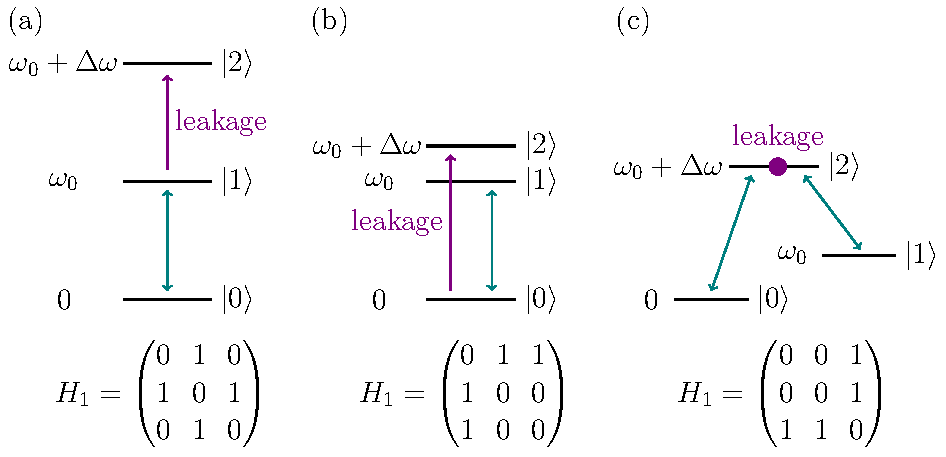
\includegraphics[width=\colfigwidth]{chapter-3-enumeration/figs/tla_leakage.pdf}
%\includestandalone[width=0.99\columnwidth]{tla_leakage}
\caption{Transitions and leakage channels included in the gate-time estimate. (a) A weakly anharmonic qubit driven directly on the $\ket{0} \rightarrow \ket{1}$ transition, with leakage through $\ket{1} \rightarrow \ket{2}$. (b) A qubit with a nearly degenerate second excited state, again driven directly on $\ket{0} \rightarrow \ket{1}$, with leakage through $\ket{0} \rightarrow \ket{2}$. (c) A Raman-type transition $\ket{0} \rightarrow \ket{2} \rightarrow \ket{1}$, where population in $\ket{2}$ is treated as leakage.} \label{fig:gate_times}
\end{figure}

\subsection{Direct Transition}
We model the qubit as a three-level system with Hamiltonian
\begin{align}
    H = H_0 + f(t)H_1 ,
\end{align}
where the free Hamiltonian is
\begin{align}
H_0 =
\begin{pmatrix}
    0 & 0 & 0 \\
    0 & \omega_0 & 0 \\
    0 & 0 & \omega_0 + \Delta\omega
\end{pmatrix} \, .
\end{align}
Here $|\Delta\omega|\geq 0$ and $\omega_0 \geq 0$, and we set the ground-state energy to zero. In \cref{fig:gate_times}, case (a) uses the drive Hamiltonian
\begin{align}
H_1 =
\begin{pmatrix}
    0 & 1 & 0 \\
    1 & 0 & 1 \\
    0 & 1 & 0
\end{pmatrix} \, .
\end{align}
The upper-left $2\times 2$ block drives the qubit $\sigma_X$ transition, while the remaining term provides a leakage channel. The relevant leakage path depends on which transition, $\ket{0}\leftrightarrow\ket{2}$ or $\ket{1}\leftrightarrow\ket{2}$, lies closer in frequency to the qubit transition $\ket{0}\leftrightarrow\ket{1}$. 

We take the drive to be a single-tone field at frequency $\omega_0$ with a Gaussian pulse envelope $f(t) = V_0 e^{-t^2/2\tau^2}\cos(\omega_0 t)$. Here $V_0$ is the peak drive amplitude. In general, the matrix elements of $H_1$, taken here to be unity, depend on the coupling scheme of the circuit.

We expect population to transfer between $\ket{0}$ and $\ket{1}$ when the pulse area is $\pi$. This corresponds to a pulse half-width of $\tau = \sqrt{\pi/2}/V_0$. By setting a maximum value for $V_0$, we obtain a minimum gate time. Faster gates, however, also increase leakage. A shorter pulse has a broader frequency spectrum, which drives the leakage transition more strongly. For weakly anharmonic systems such as the transmon, this is the main source of leakage. The DRAG protocol can suppress this effect \cite{Motzoi_DRAG_2009,Gambetta_DRAG_2009}.


To estimate leakage, we study the effective Hamiltonian:
\begin{align}
    H_\textrm{2-tone} = \begin{pmatrix}
    0 & 1 & 0 \\
    1 & 0 & \lambda \\
    0 & \lambda & 0
\end{pmatrix}\quad
\textrm{or}\quad
\begin{pmatrix}
    0 & 1 & \lambda \\
    1 & 0 & 0 \\
    \lambda & 0 & 0
\end{pmatrix}\, ,
\end{align}
with $\lambda = |F(\omega_0+\Delta\omega)/F(\omega_0)|$ or $\lambda = |F(\Delta\omega)/F(\omega_0)|$, the amplitude ratio of the Fourier transform of the drive at the leakage transition compared with the qubit transition. In chapter 9.5 of  Ref.~\cite{stancil2022principles}, it is shown that for our choice of  $f(t)$, we have
\begin{align}
    F(\omega) = \sqrt{\frac{\pi}{2}}\tau V_0(e^{-(\omega-\omega_0)^2 \tau^2/2} +e^{-(\omega+\omega_0)^2 \tau^2/2}) \, . 
\end{align}
The amplitude ratio is thus $\lambda = e^{-\delta^2 \tau^2/2}$, where $\delta$ is the detuning between the leakage transition and the qubit transition (either $\Delta\omega-\omega_0$ or $\Delta\omega$ depending on the level structure).



Solving the time-dependent Schr\"odinger equation with $\ket{\psi(t=0)} = \ket{0}$, the maximum probability to be in the $\ket{1}$ state (in both cases) is
\begin{align}
    P_{\max,\ket{1}} = \frac{1}{1+\lambda^2} = \frac{1}{1+e^{-\delta^2\tau^2}} \, .
\end{align}
To estimate the gate time, we substitute $\tau = \sqrt{\pi/2}/V_0$ corresponding to a $\pi$ pulse and solve for the $V_0$ required to achieve a population transfer of 99.9\%
\begin{align}
    \frac{1}{1+e^{-\delta^2(\sqrt{\pi/2}/V_0)^2}} = 0.999 \rightarrow V_0 \approx \frac{\delta}{2} \, .
\end{align}

Finally, we impose two drive limits. First, we assume an absolute lower bound of about 1 ns for the $\pi$-pulse width, which gives a maximum drive amplitude $V_{\rm max} = 200$ MHz. Second, we require $10 V_0 \leq \omega_0$, so that the direct drive remains within the regime described above. This gives
\begin{align}\label{eq:gtime}
\tau_{g,\textrm{direct}} =
    \begin{cases} 
      \sqrt{2\pi}/\delta, & \delta/2 \leq V_{\rm lim}\\
      \sqrt{\pi/2}/V_{\rm max} ,& \delta/2 > V_{\rm lim}
   \end{cases} \, ,
\end{align}
with $\delta$ again being the detuning between $\omega_0$ and the leakage transition ($\ket{0}\leftrightarrow\ket{2}$ or $\ket{1}\leftrightarrow\ket{2}$) and $V_{\rm lim} = \min(V_{\rm max}, \omega_0/10)$. Note that reported gate times are set to $5 \tau$, which corresponds to a pulse area of $\approx 99 \%$ of the Gaussian envelope. We see three distinct limiting factors emerge from \cref{eq:gtime}: (1) $\tau$ increases when $\delta$ is small, (2) $\tau$ increases when $\omega_0$ is small, and (3) the absolute speed limit (i.e., $\tau_{\rm min}$ is set by $V_{\rm max}$). In the case of transmon-like systems, factor (1) reproduces the conventional wisdom that gate time is inversely proportional to anharmonicity.

\subsection{Raman-Type Gate}

For transitions via $\ket{2}$, we take $H_0$ to be identical to the direct transition case, but we now consider
\begin{align}
H_1 = \begin{pmatrix}
    0 & 0 & 1 \\
    0 & 0 & 1 \\
    1 & 1 & 0
\end{pmatrix}
\end{align}
and drive the $\ket{0}\leftrightarrow\ket{2}$ and $\ket{1}\leftrightarrow\ket{2}$ transitions with
\begin{align}
    f(t) = e^{-t^2/2\tau^2}[V_1\cos(\omega_0 t - \Delta) + V_2\cos(\Delta\omega t - \Delta)] \, .
\end{align}
When the state begins in $\ket{\psi(t=0)} = \ket{0}$, it experiences Rabi oscillations between $\ket{0}$ and $\ket{1}$ with an effective Rabi frequency of $\Omega_R = V_1V_2/2\Delta$ ~\cite{gyenisMovingTransmonNoiseProtected2021b}. The intermediate state population experiences oscillations with a maximum value of 
\begin{align}
    P_{\max,\ket{2}} = \frac{V_1^2}{\Delta^2 + V_1^2 + V_2^2} \, .
\end{align}
Taking this maximum intermediate state population as a proxy for leakage, we find the $\tau$ required to limit leakage to 0.1\% (equivalent to the 99.9\% population transfer considered in the direct case). Taking $V_1 = V_2 = V$ and $\Delta = 30 V$ yields an effective Rabi frequency of $\Omega_R = V/60$, with corresponding $\tau = 60\sqrt{\pi/2}/V$ for a $\pi$ pulse. We assume here that there exists a spectrally isolated higher level state, so our only constraint is that $V \leq V_{\rm max}$. This gives $\tau$ for a Raman-style transition of
\begin{align}
    \tau_{g,\textrm{raman}} = 60\sqrt{\pi/2}/V_{\rm max}
\end{align}
Taking $V_{\rm max} = 200 \textrm{ MHz}$ as in the direct transition, we get $\tau_{g,\textrm{raman}} \approx 60$ ns. Again, the gate time is taken to be $5\tau$ to capture most of the pulse area. While $V_{\rm max}$ in the direct transition established a minimum gate time, the same constraint here establishes a maximum gate time of approximately $300$ ns.

The Raman-type gate will be preferred over the direct transition only in the cases of nearly degenerate ground states and very small anharmonicity. Due to the slow nature of these estimates, we do not consider leakage due to spectral broadening for the Raman-style transition.



% ============================================================
\section{Comparing Model with Published Results}\label{app:sweeps}
% ============================================================

To validate our model of qubit performance (e.g., \cref{eq:ngate}), we compare our predicted optimal operating points for the transmon (\texttt{JC}) and fluxonium (\texttt{JCL}) circuits with published experimental values. Including charge offset $n_g$ and external flux $\varphi_{\rm ext}$, the Hamiltonians for the two circuits are
\begin{align}
    \label{eq:tmon_flux_ham}
    % H_{\textrm{Transmon}~(\texttt{JC})} &= 4E_C (n-n_g)^2 - E_J \cos(\theta) \\
    % H_{\textrm{Transmon}~\textrm{JCL}} &= 4E_C q^2 +\frac{1}{2}E_L \varphi^2 - E_J \cos(\varphi - \varphi_{\rm ext}),
    H_{\texttt{JC}} &= 4E_C (n-n_g)^2 - E_J \cos(\theta) \\
    H_{\texttt{JCL}} &= 4E_C q^2 +\frac{1}{2}E_L \varphi^2 - E_J \cos(\varphi - \varphi_{\rm ext}) \,.
\end{align}

\begin{figure}[htbp]
\centering 
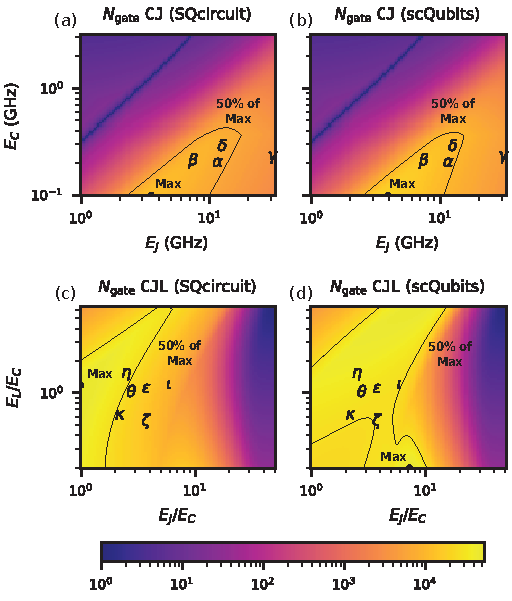
\includegraphics[width=0.5\columnwidth]{chapter-3-enumeration/figs/tmon_flux_sweep.pdf}
\caption{Qualitative estimate of $N_{\rm gate}$ calculated for the \texttt{JC} (a-b) and \texttt{JCL} (c-d) circuits. The left column (a,c) uses the \texttt{SQcircuit} noise model, which uses a second-order approximation for pure dephasing, while the right column (b,d) uses the \texttt{scQubits} noise model, which uses a first-order approximation for pure dephasing. For the \texttt{JC} circuit, $n_g = 0.25$ is chosen to represent a worst-case when a DC offset is not included. For the \texttt{JCL} circuit, the standard $\varphi_{\rm ext} = \pi$ is used, and $E_C$ is fixed at 500 MHz. The black dot marks the maximum point, and the black contour shows the region that is at least 50\% of the maximum value. The maximum value of $N_{\rm gate}$ is approximately 12,500 for the transmon (\texttt{JC}) and 54,500 for fluxonium (\texttt{JCL}). The streak with low $N_{\rm gate}$ for the \texttt{JC} circuit is due to a zero crossing of the anharmonicity. The bottom right represents the Transmon regime ($E_J/E_C \gg 1$), while the top left represents the Cooper Pair Box, or charge qubit, regime (small $E_J/E_C$). To gauge the discrepancies between our model and experimental data, we extracted the circuit parameters from various published qubit designs. Each letter corresponds to parameters from a published paper: transmon $\alpha$--\cite{krinner2022}, $\beta$--\cite{manenti_full_2021}, $\gamma$--\cite{aruteQuantumSupremacyUsing2019a}, and $\delta$--\cite{berke_transmon_2022}; fluxonium $\epsilon$--\cite{nguyen_high-coherence_2019}, $\zeta$--\cite{zhang_universal_2021}, $\eta$--\cite{bao_fluxonium_2022}, $\theta$--\cite{somoroff_fluxonium_2024}, $\iota$--\cite{somoroff2023}, and $\kappa$--\cite{moskalenko_high_2022}. Qubits from the literature fall near or within the best performing regions for both the transmon and fluxonium circuits.}
\label{fig:ngate_sweep}
\end{figure}

We visualize $N_{\rm gate}$ as a 2-D parameter sweep in \cref{fig:ngate_sweep}. In the case of fluxonium, $E_C$ is fixed at 500 MHz, with $E_L$ and $E_J$ expressed in units of $E_C$. For the transmon, $n_g = 0.25$ is chosen to represent a worst-case offset when a DC offset is not included. For fluxonium, the standard $\varphi_{\rm ext} = \pi$ is used. To provide a fair comparison with the published experimental values, we restrict our parameter ranges slightly relative to the ranges in \cref{tab:params_overview} and consider only capacitors and inductors of $E_C$ and $E_L \geq 0.1$ GHz. We use two popular software packages which have different noise models, namely \texttt{SQcircuit} \cite{rajabzadehAnalysisArbitrarySuperconducting2023,rajabzadehGeneralFrameworkGradientBased2024} and \texttt{scQubits} \cite{groszkowskiScqubitsPythonPackage2021a, chittaComputeraidedQuantizationNumerical2022a}.

In \cref{fig:ngate_sweep} (a-b) the published transmon parameters ($E_J$ and $E_C$) from the literature fall close to the 50\% contour of the numerically optimal point. The agreement is remarkable, perhaps reflecting that noise in the transmon is well understood. In the case of fluxonium, shown in \cref{fig:ngate_sweep} (c-d), the situation is more complicated.
When using the \texttt{SQcircuit} package
fewer of the published experiments fall within 50\% of our numerically optimized point. When using the \texttt{scQubits} package, the agreement improves dramatically. We believe the difference between the packages' models arises from a difference in pure dephasing rates. \texttt{SQcircuit} uses a second-order approximation, while \texttt{scQubits} uses a first-order approximation. As a result, the \texttt{SQcircuit} noise model penalizes larger $E_J$ values more due to second-order critical current noise (see \cref{fig:trans_flux_decay} for a breakdown of the individual noise channels). Nevertheless, all points except $\iota$ fall above 25\% of the maximum value for the \texttt{SQcircuit} noise model. The agreement is still impressive considering neither the noise nor gate speed models have been fine-tuned for fluxonium.


As an additional validation of the gate-time estimate in \cref{app:gate_time}, we compare our predicted gate times with the experimentally reported gate times of the reference transmon and fluxonium devices. The data are listed in \cref{tab:paper_data_tmon} and \cref{tab:paper_data_flux}. The model reproduces the ordering of the reported gate times for all devices that report one, although the variation is much smaller for the transmons. It does not predict the times exactly, but it appears to serve its intended role as a high-throughput speed limit for the optimization procedure. Somewhat surprisingly, the transmon estimates disagree more with experiment than the fluxonium estimates. One likely reason is that our target single-qubit gate coherent fidelity of 
99.9\% is lower than the 
99.99\% target relevant for the transmon devices. The context also differs: the transmon devices were integrated into a larger architecture (perhaps with e.g. DRAG pulses), whereas the fluxonium devices were more isolated research devices.




\begin{widetext}

\begin{table}[htbp]
\setlength{\tabcolsep}{3.5pt}
\footnotesize
\resizebox{\textwidth}{!}{\begin{tabular}{@{}lccccccccccc@{}}
\toprule
Group  or Device &  $E_J$ (GHz) &  $E_C$ (GHz) & $f_{01}, \eta$ (GHz) & $T_1$ ($\mu$s)& $T_2$ ($\mu$s)& $T_2^{\rm echo}$ ($\mu$s)  & $T_{\rm gate}$ (ns) & $T_{\rm gate, est}$ (ns) & $N_{\rm gate}$ \\ \toprule
% group                  | EJ    | EC     | f01, eta |  T1  | T2   | T2echo | Tgate | Ngate | Ref.

$\alpha$--\cite{krinner2022} ETH Zurich (2022) & 10.5 & 0.18  &  3.7, -0.18     &  60 &  78 & 89  & 40   & 11 & 1950  \\\midrule

$\beta$--\cite{manenti_full_2021} Rigetti (2021)   & 6.8  & 0.18  &  3.4, -0.21  &  51 &  10 & 81   & 20  & 9 &  500 \\\midrule

$\gamma$--\cite{aruteQuantumSupremacyUsing2019a} Google Sycamore (2019)  & 28.3  & 0.21  &  6.7, -0.21     &  16 &  -- & --    & 20 & 9 & 1280 \\\midrule

$\delta$--\cite{berke_transmon_2022} IBM Brooklyn (2022)  & 11.5  & 0.25  &  --     &  -- &  -- & --    & --    & -- & --   \\\midrule

\end{tabular}}
    \caption{Transmon: estimates of device parameters shown in \cref{fig:ngate_sweep}, extracted from published results. If incomplete parameters are given, we infer missing values by approximating $\eta \approx -E_C$ and $f_{01} \approx \sqrt{8 E_C E_J} - E_C$. For tunable qubits, if no idle frequency is given, we use the middle of the given range. $N_{\rm gate}$ is calculated by $N_{\rm gate} = T_2/T_{\rm gate}$. If no $T_2$ is provided, we take $1/T_2 = 1/2T_1$ -- which implies (incorrectly) that $T_{\phi}$ is infinite. For $\alpha$, we choose device D6, for $\beta$ we choose device q0, and for $\gamma$ we use the mean device parameters.}
    \label{tab:paper_data_tmon}
\end{table}

\begin{table}[htbp]
\setlength{\tabcolsep}{1pt}
\tiny
\resizebox{\textwidth}{!}{\begin{tabular}{@{}lcccccccccc@{}}
\toprule
Group  or Device &  $E_J$ (GHz) &  $E_C$ (GHz) & $E_L$ (GHz) & $f_{01}, \eta$ (GHz) & $T_1$ ($\mu$s)& $T_2$ ($\mu$s)& $T_2^{\rm echo}$ ($\mu$s)  & $T_{\rm gate}$ (ns) & $T_{\rm gate, est}$ (ns) & $N_{\rm gate}$ \\ \toprule
% group                  | EJ    | EC     |  E_L | f01, eta |  T1  | T2   | T2echo | Tgate | Tgate, est | Ngate | Ref.

$\epsilon$--\cite{nguyen_high-coherence_2019} Manucharyan (2019)   & 3.43  & 1.00  &  0.58 & 0.39, 2.84  & 500 &  510 & -- & -- & 25 & --  \\\midrule

$\zeta$--\cite{zhang_universal_2021} Schuster (2021)  &  3.40  & 0.48  &  0.13 & 0.01, 2.96  &  315 &  300 & 100   & 120 & 299 & 2500  \\\midrule

$\eta$--\cite{bao_fluxonium_2022} Alibaba (2022)   & 2.26  & 1.40  &  0.52 & 1.09, 1.93     &  80 &  35 & 30 & 10  & 9 & 3500  \\\midrule

$\theta$--\cite{somoroff_fluxonium_2024} SEEQC (2024)  &  2.50  & 0.89  &  1.14 & 1.25, 1.42  &  77 &  29.5 & 38   & 6   & 8 & 4900  \\\midrule

$\iota$--\cite{somoroff2023} Manucharyan (2023)   & 5.57  & 1.08  &  0.64 & 0.16, 5.57     &  1200 &  1160 & 1550  & 80  & 62  & 18,500  \\\midrule

$\kappa$--\cite{moskalenko_high_2022} Besedin (2022)  &  1.99  & 0.56  &  0.86 & 0.75, 1.05  &  172 &  113 & 146  & 13  & 13 & 8500  \\\midrule


\end{tabular}}
    \caption{Fluxonium: device parameters shown in \cref{fig:ngate_sweep}, extracted from published results. $N_{\rm gate}$ is calculated by $N_{\rm gate} = T_2/T_{\rm gate}$. $T_{\rm gate, est}$ represents our estimated gate time, calculated using the model described in \cref{app:gate_time}. For $\epsilon$, we choose device I, for $\eta$ we choose device A, for $\theta$ we choose device 3, and for $\kappa$ we choose device S.}
\label{tab:paper_data_flux}
\end{table}



\begin{figure*}[htbp]
\centering 
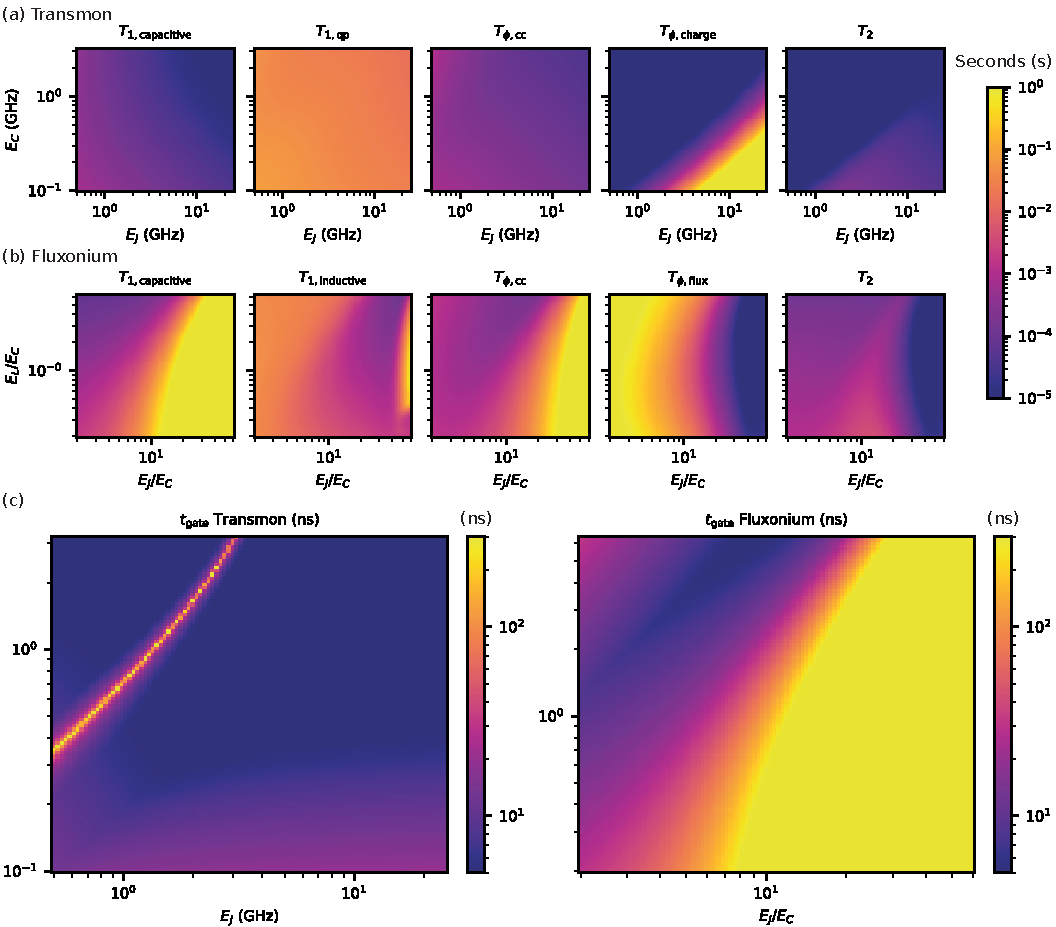
\includegraphics[width=0.99\textwidth]{chapter-3-enumeration/figs/fluxonium_noise.pdf}
\caption{Underlying coherence times and gate times estimates for the number of gates $N_{\rm gate}$ estimates in~\cref{fig:ngate_sweep}. Noise estimates from \texttt{SQcircuit} are shown for (a) transmon and (b) fluxonium. Channels not shown did not contribute meaningfully for the respective systems. Gate time estimates based on the analysis given in \cref{app:gate_time} are shown in (c). The gate time estimates for the transmon seem consistent with gate times from the literature. It is important to note that removing noises or reducing the noise magnitude will change the conclusion of our numerics.}
\label{fig:trans_flux_decay}
\end{figure*}

\FloatBarrier
\end{widetext}


\section{Optimization Results by Number of Junctions, Loops, and Compact Variables} \label{app:more_optim_results}

In \cref{tab:optim_jj,tab:optim_charge,tab:optim_loops} we split by JJs, number of charge modes, number of flux loops, respectively. Broadly speaking, these splits tell us about the relative importance of charge and flux noise when modeling the number of gates. From \cref{tab:optim_jj}, we infer that fewer JJs are preferred by our model. From \cref{tab:optim_loops}, we infer that 1 or 2 flux loops are preferred over 0, 3, or 4 loops. These preferences may be a reflection of the limited design space of three-node circuits. More flux loops means a higher sensitivity to flux noise, and with only three nodes, it is difficult to add more junctions without creating new flux loops. In \cref{tab:optim_charge}, we additionally see that compact modes are heavily penalized. Again, this may be because of the limited configurations available in three-node circuits.

\begin{table}[htbp]
\setlength{\tabcolsep}{7.5pt}
\centering
\begin{tabular}{cccc}
\toprule
$N_{JJ}$ & Circuit & $N_{\rm gate}$ (Mean) & $N_{\rm gate}$ (Std) \\ \toprule
\multirow{3}{*}{1}& \texttt{J}, \texttt{L}, \texttt{CL} & $2.77\cdot10^{5}$ & $1.6\cdot10^{4}$ \\
& \texttt{J}, \texttt{CL}, \texttt{CL} & $2.50\cdot10^{5}$ & $1.1\cdot10^{4}$ \\
& \texttt{CL}, \texttt{CL}, \texttt{CJ} & $2.38\cdot10^{5}$ & $1.1\cdot10^{4}$ \\
\midrule
\multirow{3}{*}{2}& \texttt{J}, \texttt{L}, \texttt{JL} & $2.39\cdot10^{5}$ & $1.8\cdot10^{4}$ \\
& \texttt{L}, \texttt{JL}, \texttt{CJ} & $2.36\cdot10^{5}$ & $1.1\cdot10^{4}$ \\
& \texttt{C}, \texttt{CJL}, \texttt{CJL} & $1.90\cdot10^{5}$ & $5.5\cdot10^{3}$ \\
\midrule
\multirow{3}{*}{3}& \texttt{CJ}, \texttt{CJL}, \texttt{CJL} & $1.86\cdot10^{5}$ & $3.1\cdot10^{3}$ \\
& \texttt{JL}, \texttt{JL}, \texttt{CJ} & $1.35\cdot10^{5}$ & $2.0\cdot10^{4}$ \\
& \texttt{JL}, \texttt{CJ}, \texttt{CJL} & $1.23\cdot10^{5}$ & $3.4\cdot10^{3}$ \\
\bottomrule
\end{tabular}
    \caption{Optimized number of gates for all three-node circuits, split by number of junctions $N_{JJ}$. Circuits with fewer junctions perform better than those with more junctions.} 
    \label{tab:optim_jj}
\end{table}

\begin{table}[htbp]
\setlength{\tabcolsep}{6.4pt}
\centering
\begin{tabular}{cccc}
\toprule
$N_{\rm loop}$ & Circuit & $N_{\rm gate}$ (Mean) & $N_{\rm gate}$ (Std) \\ \toprule
\multirow{2}{*}{0}& \texttt{C}, \texttt{J}, \texttt{CL} & $1.24\cdot10^{5}$ & $4.8\cdot10^{3}$ \\
& \texttt{C}, \texttt{J}, \texttt{L} & $1.22\cdot10^{5}$ & $5.6\cdot10^{3}$ \\
\midrule
\multirow{2}{*}{1}& \texttt{J}, \texttt{L}, \texttt{CL} & $2.77\cdot10^{5}$ & $1.6\cdot10^{4}$ \\
& \texttt{J}, \texttt{CL}, \texttt{CL} & $2.50\cdot10^{5}$ & $1.1\cdot10^{4}$ \\
\midrule
\multirow{2}{*}{2}& \texttt{J}, \texttt{L}, \texttt{JL} & $2.39\cdot10^{5}$ & $1.8\cdot10^{4}$ \\
& \texttt{L}, \texttt{JL}, \texttt{CJ} & $2.36\cdot10^{5}$ & $1.1\cdot10^{4}$ \\
\midrule
\multirow{2}{*}{3}& \texttt{CJ}, \texttt{CJL}, \texttt{CJL} & $1.86\cdot10^{5}$ & $3.1\cdot10^{3}$ \\
& \texttt{JL}, \texttt{JL}, \texttt{CJ} & $1.35\cdot10^{5}$ & $2.0\cdot10^{4}$ \\
\midrule
\multirow{2}{*}{4}& \texttt{CJL}, \texttt{CJL}, \texttt{CJL} & $7.04\cdot10^{4}$ & $10.0\cdot10^{2}$ \\
& \texttt{JL}, \texttt{JL}, \texttt{CJL} & $6.56\cdot10^{4}$ & $6.7\cdot10^{2}$ \\
\bottomrule
\end{tabular}
    \caption{Optimized number of gates for all three-node circuits, split by number of flux loops $N_{\rm loop}$. Circuits with one or two loops score the highest.} 
    \label{tab:optim_loops}
\end{table}

\begin{table}[htbp]
\setlength{\tabcolsep}{7.0pt}
\centering
\begin{tabular}{cccc}
\toprule
$N_{\rm compact}$ & Circuit & $N_{\rm gate}$ (Mean) & $N_{\rm gate}$ (Std) \\ \toprule
\multirow{3}{*}{0}& \texttt{J}, \texttt{L}, \texttt{CL} & $2.77\cdot10^{5}$ & $1.6\cdot10^{4}$ \\
& \texttt{J}, \texttt{CL}, \texttt{CL} & $2.50\cdot10^{5}$ & $1.1\cdot10^{4}$ \\
& \texttt{J}, \texttt{L}, \texttt{JL} & $2.39\cdot10^{5}$ & $1.8\cdot10^{4}$ \\
\midrule
\multirow{3}{*}{1}& \texttt{C}, \texttt{J}, \texttt{CJL} & $1.88\cdot10^{5}$ & $4.6\cdot10^{3}$ \\
& \texttt{C}, \texttt{CJ}, \texttt{CJL} & $1.87\cdot10^{5}$ & $3.8\cdot10^{3}$ \\
& \texttt{C}, \texttt{JL}, \texttt{CJ} & $1.87\cdot10^{5}$ & $5.1\cdot10^{3}$ \\
\midrule
\multirow{3}{*}{2}& \texttt{J}, \texttt{J}, \texttt{J} & $6.74\cdot10^{4}$ & $1.9\cdot10^{3}$ \\
& \texttt{J}, \texttt{J}, \texttt{CJ} & $6.03\cdot10^{4}$ & $1.7\cdot10^{3}$ \\
& \texttt{CJ}, \texttt{CJ} & $4.53\cdot10^{4}$ & $6.2\cdot10^{2}$ \\
\bottomrule
\end{tabular}
    \caption{Optimized number of gates for all three-node circuits, split by number of compact modes $N_{\rm compact}$. Circuits with fewer compact modes perform better.} 
    \label{tab:optim_charge}
\end{table}


\section{Circuit Quantization Details for Top Performing Circuit}\label{app:quantization_details}

\begin{figure}[htbp]
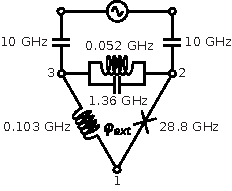
\includegraphics[width=0.5\columnwidth]{chapter-3-enumeration/figs/new_circuit_diagram.pdf}
    \caption{Circuit diagram for the top performing circuit, coupled to an AC voltage source. Each circuit node is labeled 1, 2, or 3, corresponding to node flux variables $\phi_i$.} 
    \label{fig:new_circuit_diagram}
\end{figure}


Here we derive the Hamiltonian for coupling the top-performing three-node circuit from \cref{sec:optimization} to an AC voltage source. The circuit diagram appears in \cref{fig:new_circuit_diagram}, with node labels corresponding to node-flux variables $\phi_i$.
In the node variables, the circuit has a capacitance matrix
\begin{align}
    C = \begin{pmatrix}
        C_J & -C_J & 0 \\
        -C_J & C_J + C_C + C_{23} & -C_{23} \\
        0 & -C_{23} & C_{23} + C_C
    \end{pmatrix}
\end{align}
and inverse inductance matrix
\begin{align}
    L^* = \begin{pmatrix}
        1/L_{13} & 0 & -1/L_{13} \\
        0 & 1/L_{23} & -1/L_{23} \\
        -1/L_{13} & -1/L_{23} & 1/L_{13} + 1/L_{23}
    \end{pmatrix},
\end{align}
where $L_{ij}$ and $C_{ij}$ are the inductance and capacitance between nodes $i$ and $j$. $C_J$ is the intrinsic junction capacitance and $C_C$ is the coupling capacitance to the voltage source. We do not include the effects of stray capacitance to ground, although this is included in the gate simulations of \cref{fig:new_circuit_drive}. Nodes 2 and 3 are connected to fixed-voltage nodes, giving an offset charge of
\begin{equation}
    Q_V = C_VV = \begin{pmatrix}
        0 & 0 \\
        C_c & 0 \\
        0 & C_c \\
    \end{pmatrix}\!\begin{pmatrix}
        v/2 \\
        -v/2
    \end{pmatrix} = \begin{pmatrix}
        0 \\
        C_c v/2 \\
        -C_c v/2
    \end{pmatrix}\!.
\end{equation}
Here we set the two nodes with fixed voltage to have values of $v/2$ and $-v/2$.

We choose new variables $\varphi_1 = \frac{1}{2}(\phi_3-\phi_2)$, $\varphi_2 = \phi_2-\phi_1$, and $\varphi_3 = (\phi_1 + \phi_2+\phi_3)$, which corresponds to a transformation matrix $\phi = Z\varphi$ of
\begin{align}
    Z = \begin{pmatrix}
        -2/3 & -2/3 & 1/3 \\
        -2/3 & \phantom{-}1/3 & 1/3 \\
         \phantom{-}4/3 & \phantom{-}1/3 & 1/3
    \end{pmatrix},
\end{align}
selected by the coordinate generation algorithm. After decoupling non-dynamical modes, the transformed capacitance, inductance, and charge offset matrices are
\begin{subequations}
\begin{align}
    \tilde{C} &= Z^TCZ = \begin{pmatrix}
        4 C_{23} + 2C_c & 0 & 0 \\
        0 & C_J & 0 \\
        0 & 0 & 2 C_c
    \end{pmatrix} \\
    \tilde{L}^* &= Z^TL^*Z = \begin{pmatrix}
        \frac{4(L_{13} + L_{23})}{L_{13}L_{23}} & -\frac{2}{L_{13}} & 0 \\
        -\frac{2}{L_{13}} & \frac{1}{L_{13}} & 0 \\
        0 & 0 & 0
    \end{pmatrix} \\
    \tilde{Q}_V &= Z^T C_V V = \begin{pmatrix}
        -C_c v \\
        0 \\
        0
    \end{pmatrix}.
\end{align}
\end{subequations}
The third variable is a non-dynamical free variable, uncoupled from the rest of the system, and can be ignored. The remaining two-variable $\tilde{C}$ is diagonal and can therefore be inverted trivially, yielding
\begin{align}
    \tilde{C}^{-1} &=\begin{pmatrix}
        \frac{1}{4 C_{23} + 2C_c} & 0 \\
        0 & \frac{1}{C_J}
    \end{pmatrix}.
\end{align}
After performing a Legendre transformation, we obtain the circuit Hamiltonian
\begin{align}
    H = &\frac{1}{2}(Q - \tilde{Q}_V)^T \tilde{C}^{-1}(Q - \tilde{Q}_V) \nonumber \\
        &+\frac{1}{2}\Phi^T\tilde{L}^*\Phi + U_{L}(\Phi, \Phi_{\rm ext}) +  U_{JJ}(\Phi) \nonumber \\
      = & \frac{(Q_1 + C_cV)^2}{8 C_{23} + 4C_c} + \frac{Q_2^2}{2C_J}  + \frac{2(L_{13} + L_{23})\Phi_1^2}{L_{13}L_{23}} \nonumber \\
      &- \frac{2\Phi_1\Phi_2}{L_{13}} + \frac{\Phi_2^2}{2L_{13}} \nonumber \\
      &+ \frac{2\Phi_1-\Phi_2}{L_{13}}\Phi_{\rm ext} - E_J\cos\left (\frac{2\pi}{\Phi_0}\Phi_2\right),
\end{align}
with dimension-full charge and flux variables $Q_i$ and $\Phi_i$, where $\Phi_0$ is the flux quantum. We have chosen to assign all external flux to the inductor between nodes 1 and 3 to satisfy the irrotational constraint \cite{YouKoch2019,BryonExtFlux2023}. We separate the external (drive) Hamiltonian coupled to the voltage source as 
\begin{align}
H_{\rm drive} = \frac{2C_cVQ_1}{8 C_{23} + 4C_c} = \frac{8 e^2 n_gq_1}{{8 C_{23} + 4C_c}}
\end{align}
for a dimensionless charge offset $n_g = C_cV/2e$ and charge operator $q_i = Q_i/2e$.
Here we have dropped the constant offset from the $(C_cV)^2$ term.



By examining the Hamiltonian, we see a few desirable features of this coupling scheme. First, in the ideal case, the coupling circuit drives only the first mode, whose matrix elements are large enough to enable a direct transition between $|0\rangle$ and $|1\rangle$. Second, the coupling capacitance $C_c$ adds mass to the already heavy mode while keeping the second mode light, so it only weakly perturbs the uncoupled Hamiltonian.
Lastly, coupling to the voltage source is strong, so gates can be driven with small values of $C_c V$. For the optimized pulses in \cref{fig:new_circuit_drive}, the amplitude of the control pulse $V$ is on the order of $\mu$V. Taking into account the effects of stray capacitance does mix the coupling between the two modes, but the majority of the effect remains in the first mode. Using the circuit parameters from \cref{fig:new_circuit_drive}, we have $H_{\rm drive} = n_g(g_1q_1 + g_2q_2)$, with $g_1 \approx 2.45$ GHz and $g_2 \approx 0.87$ GHz.

